\chapter{Parallelizzazione MPI}\label{cap:mpi}

Fino a questo punto il prodotto è stato descritto come se avvenisse dentro un
unico spazio di memoria: i cicli di \cref{sec:schemi} leggono $A$ e $X$ e
scrivono $Y$ come se tutte e tre fossero lì, a disposizione. Questo capitolo
rimuove quell'ipotesi. Il problema diventa far collaborare più processi che
non condividono niente, e le scelte che ne derivano condizionano tutto il
resto della relazione: la forma dei blocchi, che cosa viene cronometrato, e
perfino quali configurazioni ha senso misurare.

\section{Che cosa significa parallelizzare in MPI}\label{sec:mpi-intro}

MPI (\emph{Message Passing Interface}) è uno standard per programmare macchine
a \textbf{memoria distribuita}. Il modello di esecuzione è il seguente: lo
stesso programma viene avviato in $P$ copie, ciascuna un processo del sistema
operativo a sé stante, con il proprio spazio di indirizzi \textbf{privato}.
Nessun processo può leggere o scrivere una variabile di un altro. L'unico modo
perché un dato passi da un processo all'altro è che qualcuno lo invii
esplicitamente, con una chiamata di libreria, e qualcun altro lo riceva.

È una differenza sostanziale rispetto a un modello a memoria condivisa, dove i
thread vedono gli stessi indirizzi e la parallelizzazione consiste
essenzialmente nel ripartire le iterazioni di un ciclo. Qui ripartire le
iterazioni non basta, e non è nemmeno la prima cosa da decidere: prima bisogna
stabilire \textbf{chi possiede quale dato}. Da questa scelta discende tutto il
resto, perché un processo può calcolare solo ciò per cui possiede gli
ingredienti, e ogni ingrediente mancante è un messaggio da far viaggiare.

La parallelizzazione del nucleo si articola quindi in tre domande, in
quest'ordine:

\begin{enumerate}[nosep,left=0pt]
  \item \textbf{decomposizione} - come si tagliano $A$, $X$ e $Y$ fra i
        processi;
  \item \textbf{località} - quale parte del risultato ciascun processo riesce
        a calcolare con i soli dati che possiede;
  \item \textbf{comunicazione} - che cosa manca, e in quale direzione deve
        viaggiare perché il risultato locale diventi il risultato giusto.
\end{enumerate}

\begin{itemize}[nosep,left=0pt]
  \item Il \textbf{rank} è l'identificatore intero di un processo all'interno
        di un gruppo: è ciò che permette a un programma unico di comportarsi
        diversamente su processi diversi.
  \item Un \textbf{comunicatore} è un gruppo di processi assieme a un contesto
        di comunicazione isolato. Ogni operazione MPI avviene \emph{dentro} un
        comunicatore, e i rank hanno senso solo rispetto a quello:
        \code{MPI\_COMM\_WORLD} è il comunicatore predefinito che contiene
        tutti i processi, ma se ne possono costruire altri più piccoli, ed è
        esattamente ciò che il progetto fa.
  \item Un'operazione \textbf{collettiva} è un'operazione che tutti i processi
        di un comunicatore devono chiamare. Il progetto ne usa due:
        il \emph{broadcast}, in cui un processo possiede un dato e al termine
        lo possiedono tutti; e la \emph{reduce}, in cui ogni processo possiede
        un array della stessa forma, gli array vengono combinati elemento per
        elemento con un operatore associativo --- qui la somma --- e il
        risultato finisce su un solo processo.
  \item Il \textbf{root} è quel processo designato: la sorgente nel broadcast,
        il destinatario nella reduce.
\end{itemize}

\section{Perché si taglia \texorpdfstring{$A$}{A}, e perché in due direzioni}
\label{sec:perche-2d}

\subsection{Che cosa tagliare}

La prima decisione riguarda quale delle tre matrici vada distribuita. La
risposta viene da \cref{sec:traffico}: $A$ ha $MN$ elementi, $X$ e $Y$ ne
hanno rispettivamente $Nk$ e $Mk$, e con $k$ piccolo per definizione $A$ è più
grande delle altre due di un fattore che cresce con la taglia del problema.

Replicare $A$ su ogni processo sarebbe quindi la scelta peggiore possibile, e
per due ragioni indipendenti: ogni nodo dovrebbe contenerla per intero,
mettendo un tetto alla taglia massima trattabile a prescindere da quanti
processi si usino; e ogni processo la rileggerebbe tutta, quando è proprio il
traffico su $A$ a determinare il tempo. $A$ va dunque \textbf{tagliata}. $X$ e
$Y$, che sono piccole, possono invece permettersi di essere replicate lungo un
asse, e vedremo che è esattamente ciò che conviene fare.

\subsection{Come tagliare: due possibilità monodimensionali}

Tagliare $A$ significa assegnare a ogni processo una sottomatrice. Le
decomposizioni più semplici la tagliano lungo una sola dimensione, e la
\cref{eq:definizione} dice subito che cosa comportano.

\paragraph{Taglio a bande di righe.} Ogni processo possiede righe \emph{intere}
di $A$. Per calcolare $Y[i][c]$ serve tutta la riga $i$ di $A$ e tutte le
righe di $X$: un processo che possiede righe intere possiede quindi tutti i
fattori del primo tipo, ma gli serve $X$ per intero. Il vantaggio è che il
risultato che calcola è già \emph{definitivo}: nessuna somma finale fra
processi. Il costo è che $X$ deve essere replicata su tutti i $P$ processi.

\paragraph{Taglio a bande di colonne.} Ogni processo possiede colonne di $A$,
cioè, per ciascuna riga, solo una parte degli addendi della sommatoria. Gli
basta quindi la porzione di $X$ corrispondente alle proprie colonne --- $X$
viene tagliata e non replicata --- ma ciò che produce è un risultato
\textbf{parziale}, che riguarda tutte le righe di $Y$ e va sommato con i
parziali di tutti gli altri. La somma finale coinvolge $P$ processi su un
oggetto della taglia piena di $Y$.

\medskip

Le due alternative sono speculari: la prima paga la replicazione di $X$ su
tutti, la seconda la riduzione di $Y$ su tutti. In entrambe la comunicazione
coinvolge sempre l'intero insieme dei processi, e questo è il difetto
strutturale: aumentare $P$ non rende i messaggi più piccoli, li rende soltanto
più numerosi.

\subsection{Il taglio bidimensionale}

La terza possibilità taglia $A$ in entrambe le direzioni: ogni processo
possiede un \emph{rettangolo} della matrice. Le due necessità di prima
compaiono ora entrambe --- servono le righe di $X$ corrispondenti alle proprie
colonne di $A$, e il proprio contributo a $Y$ è parziale e va sommato --- ma
ciascuna coinvolge soltanto un \textbf{sottoinsieme} dei processi: quelli che
condividono le stesse colonne di $A$ per la prima, quelli che condividono le
stesse righe per la seconda. Nessuna delle due comunicazioni è più globale.

È questa la decomposizione richiesta dalla traccia, ed è quella che il progetto
implementa. Che sia effettivamente superiore alle due monodimensionali non è
però qualcosa da accettare sulla fiducia: è una proprietà quantificabile, e la
\cref{sec:modello-comunicazione} la dimostra con un modello di costo,
mostrando che le due decomposizioni 1D ne sono i casi degeneri. Il confronto
viene poi misurato direttamente in \cref{cap:risultati}.


% ---------------------------------------------------------------------------
% Figura: taglio bidimensionale di A, con X e Y tagliate lungo una sola
% dimensione. Da inserire in sezioni/04-mpi.tex, in \cref{sec:perche-2d}.
% ---------------------------------------------------------------------------
\begin{figure}[H]
\centering
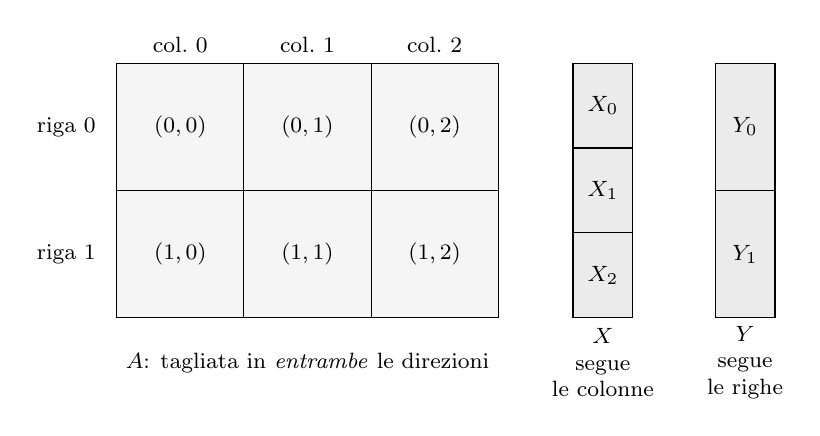
\begin{tikzpicture}[scale=0.95,every node/.style={font=\footnotesize}]

  % --- A: griglia 2 x 3 di blocchi -----------------------------------------
  \foreach \r in {0,1} {
    \foreach \c in {0,1,2} {
      \draw[fill=black!4] (\c*1.7,-\r*1.7) rectangle ++(1.7,1.7);
      \node at (\c*1.7+0.85,-\r*1.7+0.85) {$(\r,\c)$};
    }
  }
  % etichette di riga e colonna della griglia
  \node[anchor=east] at (-0.15,0.85)  {riga 0};
  \node[anchor=east] at (-0.15,-0.85) {riga 1};
  \node at (0.85,1.95) {col.\ 0};
  \node at (2.55,1.95) {col.\ 1};
  \node at (4.25,1.95) {col.\ 2};
  \node at (2.55,-2.3) {$A$: tagliata in \emph{entrambe} le direzioni};

  % --- X: tagliata per bande di righe, una per banda di colonne di A -------
  \foreach \b in {0,1,2} {
    \draw[fill=black!8] (6.1,1.7-\b*1.133) rectangle ++(0.8,-1.133);
    \node at (6.5,1.7-\b*1.133-0.567) {$X_{\b}$};
  }
  \node[align=center] at (6.5,-2.3) {$X$\\segue\\le colonne};

  % --- Y: tagliata per bande di righe, una per banda di righe di A ---------
  \foreach \b in {0,1} {
    \draw[fill=black!8] (8.0,1.7-\b*1.7) rectangle ++(0.8,-1.7);
    \node at (8.4,1.7-\b*1.7-0.85) {$Y_{\b}$};
  }
  \node[align=center] at (8.4,-2.3) {$Y$\\segue\\le righe};

\end{tikzpicture}
\caption{Decomposizione dei dati su una griglia $2 \times 3$. Ogni processo
possiede un \emph{rettangolo} di $A$, individuato dalle sue coordinate nella
griglia. Il multivettore $X$ \`e tagliato per bande di righe, una per ciascuna
banda di colonne di $A$; $Y$ per bande di righe, una per ciascuna banda di
righe di $A$. Nessuna delle due \`e mai tagliata lungo $k$.}
\label{fig:taglio-2d}
\end{figure}

\subsection{Perché i processi vengono organizzati a griglia}

Resta un ultimo passaggio, che è di comodità ma non solo. Se il taglio del
dato è bidimensionale, conviene che lo sia anche il modo in cui si identificano
i processi: un processo individuato da una coppia di coordinate
$(r, c)$ invece che da un intero rende immediate le due relazioni che servono
di continuo. «I processi che possiedono le stesse colonne di $A$» diventa «i
processi della stessa colonna della griglia», e non un calcolo aritmetico sui
rank da rifare ogni volta.

MPI offre questa struttura nativamente, sotto il nome di \textbf{topologia
virtuale cartesiana}. È virtuale nel senso che non descrive come i nodi sono
fisicamente cablati: descrive come il programma vuole \emph{pensare}
all'insieme dei propri processi, lasciando però all'implementazione la
possibilità di sfruttare quell'informazione per disporli meglio sulla macchina
reale.

\section{Decomposizione a griglia bidimensionale}
\label{sec:griglia}

I $P$ processi vengono organizzati in una griglia cartesiana
$\Prow \times \Pcol = P$, costruita con \code{MPI\_Cart\_create}. La chiamata
restituisce un nuovo comunicatore nel quale ogni processo ha, oltre al proprio
rank, una coppia di coordinate recuperabile con \code{MPI\_Cart\_coords}: sono
le $(r,c)$ della sezione precedente, ed è su di esse che il codice ragiona da
qui in avanti.

Due parametri della chiamata meritano una nota:

\begin{itemize}[nosep,left=0pt]
  \item la griglia è dichiarata \textbf{non periodica}. La periodicità serve
        agli schemi in cui ogni processo comunica con i propri vicini e il
        bordo deve richiudersi sul lato opposto; qui le comunicazioni sono
        collettive lungo un'intera riga o colonna, e un collegamento fra
        l'ultimo processo e il primo non avrebbe alcun significato;
  \item \code{reorder = 1} autorizza l'implementazione a \textbf{rinumerare}
        i processi rispetto a \code{MPI\_COMM\_WORLD}, per far corrispondere
        meglio la griglia logica alla topologia fisica della macchina. È la
        libertà che rende utile una topologia virtuale, ma ha una conseguenza
        da non dimenticare: da quel momento l'unico rank valido è quello del
        nuovo comunicatore, e assumere che coincida con quello di partenza
        sarebbe un errore.
\end{itemize}

La forma della griglia può essere imposta dall'utente con i flag \code{--pr} e
\code{--pc}. In assenza di indicazione, \code{grid\_default\_shape} sceglie la
fattorizzazione più vicina alla forma quadrata, prendendo come $\Prow$ il più
grande divisore di $P$ non superiore a $\sqrt{P}$; ne segue
$\Prow \le \Pcol$, e nel caso limite di $P$ primo la griglia degenera in
$1 \times P$. La ragione per cui il quadrato è un buon default, e i casi in cui
non lo è, sono in \cref{sec:modello-comunicazione}.


\subsection{I due sotto-comunicatori}

La griglia da sola non basta: le collettive vanno eseguite lungo una riga o
lungo una colonna, non sull'insieme di tutti i processi, e una collettiva
agisce su un comunicatore intero. Servono quindi comunicatori più piccoli, uno
per ogni riga e uno per ogni colonna della griglia.

Li produce \code{MPI\_Cart\_sub}, a cui si indica quali dimensioni lasciar
variare e quali tenere fisse. Fissando la coordinata di riga e lasciando
variare quella di colonna si ottiene \code{row\_comm}, che raccoglie i
processi di una stessa \emph{riga}; fissando la colonna si ottiene
\code{col\_comm}, che raccoglie quelli di una stessa \emph{colonna}. Ogni
processo appartiene esattamente a un \code{row\_comm} e a un \code{col\_comm},
e sono i due assi lungo cui viaggiano le uniche due collettive del cammino
cronometrato.

\subsection{Chi fa da root, e perché la scelta è verificata}

Entrambe le collettive hanno bisogno di un root, e in entrambi i casi il
processo giusto è determinato dal problema, non arbitrario: il broadcast di
$X$ deve partire dal processo di riga $0$, che è l'unico a possedere
inizialmente quella fetta, e la reduce di $Y$ deve arrivare al processo di
colonna $0$, che è il proprietario designato di quella porzione del risultato.


\begin{figure}[H]
\centering
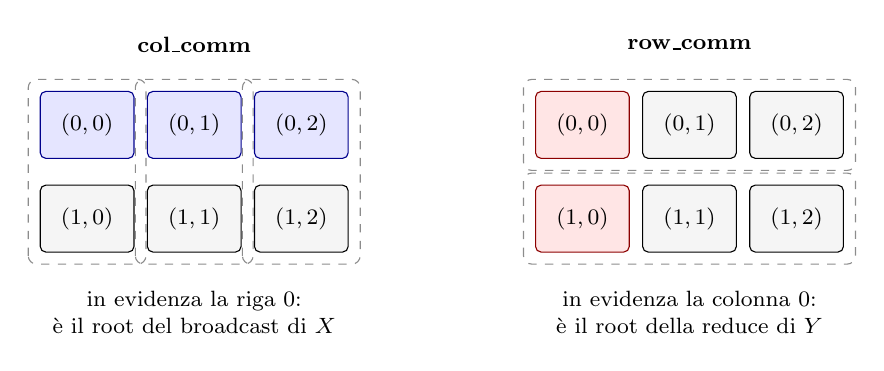
\begin{tikzpicture}[scale=0.85,every node/.style={font=\footnotesize},
                    gruppo/.style={draw=black!45,dashed,rounded corners=3pt},
                    cella/.style={rounded corners=2pt}]
  \begin{scope}
    \foreach \cl in {0,1,2} {
      \draw[cella,fill=blue!10,draw=blue!55!black] (\cl*1.6,0) rectangle ++(1.4,1.0);
      \node at (\cl*1.6+0.7,0.5) {$(0,\cl)$};
    }
    \foreach \cl in {0,1,2} {
      \draw[cella,fill=black!4] (\cl*1.6,-1.4) rectangle ++(1.4,1.0);
      \node at (\cl*1.6+0.7,-0.9) {$(1,\cl)$};
    }
    \foreach \cl in {0,1,2} {
      \draw[gruppo] (\cl*1.6-0.18,-1.58) rectangle (\cl*1.6+1.58,1.18);
    }
    \node[font=\footnotesize\bfseries] at (2.3,1.7) {\code{col\_comm}};
    \node[align=center] at (2.3,-2.3)
      {in evidenza la riga 0:\\è il root del broadcast di $X$};
  \end{scope}
  \begin{scope}[xshift=7.4cm]
    \foreach \rw in {0,1} {
      \draw[cella,fill=red!10,draw=red!55!black] (0,-\rw*1.4) rectangle ++(1.4,1.0);
      \node at (0.7,-\rw*1.4+0.5) {$(\rw,0)$};
    }
    \foreach \rw in {0,1} {
      \foreach \cl in {1,2} {
        \draw[cella,fill=black!4] (\cl*1.6,-\rw*1.4) rectangle ++(1.4,1.0);
        \node at (\cl*1.6+0.7,-\rw*1.4+0.5) {$(\rw,\cl)$};
      }
    }
    \foreach \rw in {0,1} {
      \draw[gruppo] (-0.18,-\rw*1.4-0.18) rectangle (4.78,-\rw*1.4+1.18);
    }
    \node[font=\footnotesize\bfseries] at (2.3,1.7) {\code{row\_comm}};
    \node[align=center] at (2.3,-2.3)
      {in evidenza la colonna 0:\\è il root della reduce di $Y$};
  \end{scope}
\end{tikzpicture}
\caption{La stessa griglia, raggruppata nei due modi. Fissando la coordinata di
riga si ottengono i comunicatori \code{row\_comm}, fissando quella di colonna i
comunicatori \code{col\_comm}. Ogni processo appartiene a esattamente uno di
ciascun tipo, e i due si intersecano soltanto in lui.}
\label{fig:sottocomunicatori}
\end{figure}


Indicare il root a una collettiva significa però indicarne il \emph{rank nel
sotto-comunicatore}, non le coordinate nella griglia. Il codice sfrutta allora
una proprietà di \code{MPI\_Cart\_sub}: in un sotto-comunicatore con una sola
dimensione residua i rank risultano ordinati per coordinata crescente. Ne segue
che il rank $0$ di \code{col\_comm} è il processo di riga $0$, e il rank $0$ di
\code{row\_comm} è il processo di colonna $0$: in entrambi i casi il root
cercato, e le due collettive possono usare semplicemente $0$.

La proprietà viene comunque \textbf{verificata} in \code{grid\_create},
confrontando il rank in ciascun sotto-comunicatore con la coordinata
cartesiana corrispondente. Il motivo è la libertà concessa da
\code{reorder = 1}: se l'ipotesi cadesse, le collettive continuerebbero a
funzionare regolarmente, ma con il root sbagliato, e il programma produrrebbe
risultati errati senza segnalare nulla.

\section{Partizionamento degli indici}
\label{sec:indici}

Decidere la forma della griglia non basta: bisogna ancora stabilire, per
ciascuna delle due dimensioni, quali indici globali finiscano su quale parte.
La regola è una sola e viene applicata due volte --- alle righe di $A$ fra le
$\Prow$ righe della griglia, alle colonne fra le $\Pcol$ colonne --- ed è una
partizione \textbf{a blocchi}: ogni parte riceve un intervallo contiguo di
indici, e il resto della divisione viene distribuito un elemento per volta
sulle prime parti.

Il blocco contiguo non è una scelta di comodo. L'alternativa naturale sarebbe
una distribuzione ciclica, che assegna gli indici a turno; ma qui il lavoro per
elemento è uniforme, quindi il ciclico non bilancerebbe nulla che il blocco già
non bilanci, e in cambio distruggerebbe la contiguità --- cioè proprio la
proprietà da cui dipendono sia il datatype derivato della distribuzione
(\cref{sec:distribuzione-a}) sia il passo unitario degli accessi dello schema~A
(\cref{sec:schemi}).

\subsection{Le funzioni}

Posti $q = \lfloor n/p \rfloor$ e $r = n \bmod p$, le prime $r$ parti hanno
$q+1$ elementi e le restanti $q$. Da qui le prime due funzioni, che dicono
\emph{quanti} elementi tocchino alla parte $i$ e \emph{da dove} cominci:

\begin{equation}
  \mathrm{size}(n,p,i) = q +
      \begin{cases} 1 & i < r\\ 0 & \text{altrimenti}\end{cases}
  \qquad
  \mathrm{start}(n,p,i) = i\,q + \min(i,\ r).
  \label{eq:partizione}
\end{equation}

Il $\min(i,r)$ nell'offset conta quante parti \emph{lunghe} precedono la parte
$i$: finché $i < r$ sono tutte lunghe e se ne accumula una per ciascuna, dopo
il loro numero resta fermo a $r$. La funzione è definita anche per $i = p$,
dove vale $n$: una sentinella che rende l'ultima parte un caso come gli altri.

Lo sbilanciamento massimo è di un elemento per dimensione: fra due blocchi
locali qualsiasi c'è al più una riga e una colonna di differenza.

\section{Layout dei blocchi locali}
\label{sec:layout}

Applicando la partizione alle due dimensioni si ottiene la forma dei tre
blocchi che ogni processo possiede:
\begin{equation}
  A_{\text{loc}} : \mloc \times \nloc,
  \qquad
  X_{\text{loc}} : \nloc \times k,
  \qquad
  Y_{\text{loc}} : \mloc \times k,
\end{equation}
con $\mloc = \mathrm{size}(M, \Prow, \code{my\_row})$ e
$\nloc = \mathrm{size}(N, \Pcol, \code{my\_col})$.

\subsection{Perché i conteggi delle collettive tornano}

Nelle due formule qui sopra c'è una proprietà che vale la pena rendere
esplicita, perché è la condizione di consistenza delle due collettive:
$\mloc$ dipende \textbf{solo} da \code{my\_row} e $\nloc$ \textbf{solo} da
\code{my\_col}.

Ne segue che tutti i processi di una stessa riga della griglia concordano su
$\mloc$, e tutti quelli di una stessa colonna concordano su $\nloc$. Sono
esattamente i due gruppi su cui agiscono le collettive: il broadcast lungo
\code{col\_comm} usa un conteggio di $\nloc \cdot k$ elementi, e i suoi
partecipanti condividono la colonna, dunque $\nloc$; la reduce lungo
\code{row\_comm} usa $\mloc \cdot k$, e i suoi partecipanti condividono la
riga, dunque $\mloc$. Nessuno dei due conteggi va negoziato o comunicato: viene
dalla stessa formula, valutata su coordinate che i partecipanti hanno in
comune.

\subsection{Chi contiene che cosa, e quando}

Il buffer $X_{\text{loc}}$ esiste su \emph{tutti} i processi --- il broadcast
deve avere dove scrivere --- ma prima del broadcast contiene dati significativi
soltanto sui processi della riga $0$. Dopo il prodotto locale ogni processo
possiede un contributo \emph{parziale} a $Y$, che riguarda le proprie righe ma
soltanto le proprie colonne di $A$; la \code{MPI\_Reduce} lungo
\code{row\_comm} li somma e produce il blocco definitivo sui processi della
colonna $0$.

\subsection{Perché il multivettore non viene mai tagliato lungo \texorpdfstring{$k$}{k}}

Le $k$ colonne restano indivise su tutti i processi. Tre ragioni, in ordine di
peso:

\begin{itemize}[nosep,left=0pt]
  \item \textbf{costringerebbe a replicare $A$.} Per calcolare un qualunque
        sottoinsieme di colonne di $Y$ serve comunque \emph{tutta} $A$: i
        processi di una stessa partizione lungo $k$ vorrebbero perciò lo stesso
        identico blocco di $A$. Si duplicherebbe il dato dominante, che è l'opposto di ciò per cui la decomposizione
        esiste;
  \item \textbf{ridurrebbe il riuso di $A$ in registro.} Nello schema~A il
        fattore di riuso è pari al numero di colonne che il processo possiede
        localmente (\cref{sec:schemi}): frazionare $k$ lo frazionerebbe nella
        stessa misura, abbassando l'intensità aritmetica del nucleo;
  \item \textbf{produrrebbe messaggi troppo piccoli.} $k$ è piccolo per
        definizione del problema, e frammentarlo ulteriormente darebbe
        comunicazioni dominate dalla latenza invece che dalla banda.
\end{itemize}

\section{Distribuzione iniziale dei dati}
\label{sec:distribuzione-a}

Le modalit\`a di inizializzazione di $A$ e $X$ sono indipendenti
(\code{--a-mode}, \code{--x-mode}), e tutte e quattro le combinazioni sono
valide. Le due modalità di ciascuna matrice producono gli stessi elementi
globali a parità di seed, per la proprietà del generatore discussa in
\cref{sec:generazione}.

\paragraph{\code{--a-mode global}.} Il grid rank $0$ materializza $A$ completa e
la distribuisce. È il caso interessante dal punto di vista MPI: i sottoblocchi
2D \textbf{non sono contigui} nella matrice row-major globale. Il mittente
descrive il blocco da inviare con un \code{MPI\_Type\_vector} di $\mloc$ blocchi
da $\nloc$ elementi e stride $N$. Il destinatario ne descrive uno con stride \code{lda}, che può essere diverso:
è il caso generale - due layout differenti sui due lati della stessa
comunicazione - e non richiede nessun buffer intermedio né nessuna copia
manuale. Il rank $0$ fa eccezione per il proprio blocco, che copia
direttamente senza passare da MPI.

\paragraph{\code{--a-mode local}.} Ogni processo genera direttamente il proprio blocco 2D di 
$A$ dagli indici globali. In questo modo non è necessario materializzare una copia globale
aggiuntiva della matrice su un singolo processo.


\paragraph{\code{--x-mode global}} Il
grid rank $0$ materializza la $X$ compatta $N \times k$ e un
\code{MPI\_Scatterv} sul \code{row\_comm} della riga $0$ ne distribuisce i blocchi di righe:
entrambi i lati sono contigui, perché $\code{ldx} = k$ ovunque, quindi non
serve nessun datatype derivato. 

\paragraph{\code{--x-mode local}} I processi
della riga $0$ generano direttamente le proprie righe di $X$. Il successivo broadcast lungo \code{col\_comm}
è identico alla modalità \code{global}.

\medskip

Generazione e distribuzione iniziale fanno parte del \textbf{preprocessing},
perciò sono escluse dai tempi ufficiali.
La modalità \code{global} rappresenta uno scenario in cui l'input è inizialmente centralizzato.

\section{L'algoritmo distribuito}

Un'invocazione del prodotto esegue tre passi:

\begin{lstlisting}[language=C,caption={Il corpo di \code{mpi\_matmul}, senza i cronometri.}]
MPI_Bcast(X_loc, n_loc*k, SCALAR_MPI_TYPE, 0, grid->col_comm);

local_gemm(local_gemm_context, X_loc, layout->ldx, Y_loc_part, layout->ldy);

MPI_Reduce(Y_loc_part, Y_row_col0, m_loc*k, SCALAR_MPI_TYPE,
           MPI_SUM, 0, grid->row_comm);
\end{lstlisting}

\begin{enumerate}[nosep,left=0pt]
  \item \textbf{Broadcast di $X$ lungo \code{col\_comm}:} tutti i processi di una
        colonna della griglia lavorano sulle stesse colonne di $A$, quindi
        servono loro le stesse righe di $X$. Il root è il processo di riga $0$,
        l'unico che possiede inizialmente quella fetta, ne è il \emph{responsabile}.
  \item \textbf{Prodotto locale:} il risultato \`e \emph{parziale}: il processo
        in posizione $(r,c)$ calcola il contributo delle sole colonne
        $[\text{col}_0, \text{col}_0 + \nloc)$ di $A$ alle righe
        $[\text{row}_0, \text{row}_0 + \mloc)$ di $Y$ (dove $\text{row}_0$ e $\text{col}_0$ sono gli offset globali del blocco locale).
  \item \textbf{Reduce lungo \code{row\_comm}:} i $\Pcol$ contributi parziali
        della stessa banda di righe vivono sui processi di una stessa riga della
        griglia: sommandoli tra loro si ottiene $Y$.
        
        Il \code{count} \`e $\mloc \cdot k$
        (e non $1$) dato che la riduzione agisce lungo la dimensione dei processi e
        preserva la posizione, producendo dunque $\mloc \cdot k$ somme indipendenti.
        
        Il root è il processo di colonna $0$, che è già il \emph{responsabile} designato
        di quella porzione di $Y$: nessuna ridistribuzione finale è necessaria.
\end{enumerate}



\begin{figure}[H]
\centering
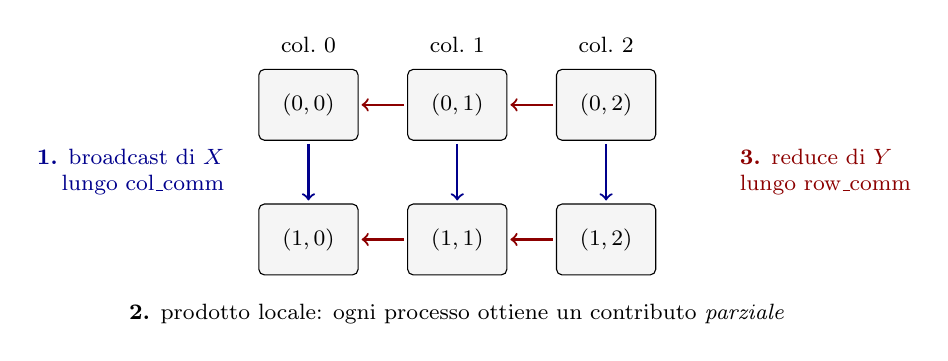
\begin{tikzpicture}[scale=0.9,every node/.style={font=\footnotesize},
                    cella/.style={rounded corners=2pt,fill=black!4},
                    bcast/.style={->,thick,blue!55!black},
                    reduce/.style={->,thick,red!55!black}]

  % --- celle della griglia 2 x 3 -------------------------------------------
  \foreach \cl in {0,1,2} {
    \draw[cella] (\cl*2.1,0) rectangle ++(1.4,1.0);
    \node at (\cl*2.1+0.7,0.5) {$(0,\cl)$};
    \draw[cella] (\cl*2.1,-1.9) rectangle ++(1.4,1.0);
    \node at (\cl*2.1+0.7,-1.4) {$(1,\cl)$};
  }
  \node at (0.7,1.35) {col.\ 0};
  \node at (2.8,1.35) {col.\ 1};
  \node at (4.9,1.35) {col.\ 2};

  % --- passo 1: broadcast di X, lungo le colonne ---------------------------
  \foreach \cl in {0,1,2} {
    \draw[bcast] (\cl*2.1+0.7,-0.05) -- (\cl*2.1+0.7,-0.85);
  }
  \node[anchor=east,align=right,blue!55!black] at (-0.35,-0.45)
    {\textbf{1.} broadcast di $X$\\lungo \code{col\_comm}};

  % --- passo 3: reduce di Y, lungo le righe verso la colonna 0 -------------
  \foreach \rw in {0,1} {
    \draw[reduce] (2.05,-\rw*1.9+0.5) -- (1.45,-\rw*1.9+0.5);
    \draw[reduce] (4.15,-\rw*1.9+0.5) -- (3.55,-\rw*1.9+0.5);
  }
  \node[anchor=west,align=left,red!55!black] at (6.65,-0.45)
    {\textbf{3.} reduce di $Y$\\lungo \code{row\_comm}};

  % --- passo intermedio: il prodotto locale --------------------------------
  \node at (2.8,-2.45) {\textbf{2.} prodotto locale: ogni processo ottiene un contributo \emph{parziale}};

\end{tikzpicture}
\caption{Le due collettive di una singola invocazione. Il broadcast fa scendere
la fetta di $X$ dal processo di riga $0$ a tutti i processi della sua colonna,
che ne hanno bisogno perché condividono le stesse colonne di $A$. Dopo il
prodotto locale ogni processo possiede un contributo \emph{parziale} a $Y$: la
reduce somma i $\Pcol$ parziali di una stessa banda di righe e deposita il
risultato sul processo di colonna $0$, che ne è il proprietario designato.}
\label{fig:collettive}
\end{figure}

\section{Modello di costo della comunicazione}
\label{sec:modello-comunicazione}

Il costo di un messaggio di $n$ byte fra due processi si modella, seguendo le
dispense del corso, come
\begin{equation}
  T(n) \;=\; \lambda + \frac{n}{B},
  \label{eq:costo-messaggio}
\end{equation}
dove $\lambda$ è la \emph{latenza}, un costo fisso che si paga per ogni
messaggio indipendentemente dalla sua taglia, e $B$ è la \emph{banda}. In
letteratura lo stesso modello compare spesso nella forma $\alpha + \beta n$:
il dizionario è $\alpha \equiv \lambda$ e $\beta \equiv 1/B$.

Le due collettive non sono però messaggi singoli. Il costo logaritmico che
segue è quello del \emph{recursive doubling}, l'algoritmo di broadcast visto a
lezione, che al posto dei $p-1$ invii sequenziali della versione ingenua
costa $T(p) = \lceil \log_2 p \rceil$ tempi di messaggio. Il logaritmo si
ottiene grazie a un'ipotesi precisa sulla rete - che essa sostenga più
messaggi contemporaneamente, purché le coppie di nodi coinvolte non si
sovrappongano - ed è quell'ipotesi, più che la struttura ad albero, a
rendere possibile il guadagno.

Detti $s$ i byte per scalare, il costo di comunicazione per invocazione è
quindi
\begin{equation}
  T_{\text{comm}} \;\approx\;
  \underbrace{\lceil\log_2 \Prow\rceil
     \Bigl(\lambda + \frac{s\,k\,N/\Pcol}{B}\Bigr)}_{\text{broadcast di } X}
  \;+\;
  \underbrace{\lceil\log_2 \Pcol\rceil
     \Bigl(\lambda + \frac{s\,k\,M/\Prow}{B} + \gamma\,k\,\frac{M}{\Prow}\Bigr)}_{\text{reduce di } Y},
  \label{eq:costo-comm}
\end{equation}
dove $\gamma$ è il costo per elemento della somma eseguita dalla reduce. Il
termine in $\gamma$ non compare nel modello del corso, che descrive il costo
del solo trasferimento: lo aggiungiamo perché la reduce, a differenza del
broadcast, a ogni livello dell'albero esegue anche $\mloc \cdot k$ addizioni.

Il modello va letto per quello che è: i fattori logaritmici valgono se
l'implementazione usa il recursive doubling, ma le librerie MPI cambiano algoritmo
al crescere del messaggio e per messaggi grandi passano a schemi a pipeline o
scatter/allgather, nei quali il termine di banda perde il fattore logaritmico e
resta proporzionale al solo volume trasferito.

Il modello va letto per quello che è: i fattori logaritmici valgono se
l'implementazione usa il recursive doubling, ma --- come le dispense stesse
osservano --- una buona libreria MPI commuta internamente fra algoritmi
diversi a seconda dell'operazione, della rete e soprattutto della quantità di
dati. Per messaggi grandi si passa a schemi a pipeline o scatter/allgather,
nei quali ogni byte attraversa la rete una volta sola invece di $\log_2 p$
volte: il termine di banda perde il fattore logaritmico e resta proporzionale
al solo volume, al prezzo di un numero maggiore di messaggi e quindi di più
latenza.

Alle taglie della campagna i
messaggi cadono in quel regime, quindi il $\log_2$ va inteso come limite
superiore sui termini di latenza più che come andamento atteso della banda.
Questo non intacca però la conclusione che segue: il \emph{volume}, cioè
l'unica quantità da cui dipende la scelta della forma della griglia, è lo
stesso per qualunque algoritmo collettivo, perché è quanto ciascun processo
deve comunque ricevere o inviare.

Il termine che decide la forma ottima della griglia \`e il volume:
\begin{equation}
  V(\Prow,\Pcol) \;=\; k\Bigl(\frac{N}{\Pcol} + \frac{M}{\Prow}\Bigr),
  \qquad \Prow \Pcol = P .
  \label{eq:volume}
\end{equation}
Minimizzando con il vincolo $\Prow\Pcol = P$ si ottiene
\begin{equation}
  \Prow^{\star} = \sqrt{P\,\frac{M}{N}},
  \qquad
  \Pcol^{\star} = \sqrt{P\,\frac{N}{M}},
  \qquad
  V^{\star} = \frac{2k\sqrt{MN}}{\sqrt{P}} .
  \label{eq:ottimo}
\end{equation}

Due letture, entrambe verificate sperimentalmente in \cref{cap:risultati}:

\begin{itemize}[nosep,left=0pt]
  \item \textbf{Perch\'e 2D e non 1D.} Le due decomposizioni monodimensionali
        sono i casi degeneri $\Prow = 1$ (volume $kM$, nessun broadcast ma
        reduce su tutti i $P$ processi) e $\Pcol = 1$ (volume $kN$, nessuna
        reduce ma broadcast su tutti i $P$). In entrambi il volume \emph{non
        decresce} con $P$, mentre la griglia 2D lo fa scendere come
        $1/\sqrt{P}$. \`E il motivo per cui la traccia richiede una griglia
        bidimensionale, ed \`e ci\`o che la campagna C6 misura direttamente
        confrontando tutte le fattorizzazioni di $P$, forme degeneri comprese.
  \item \textbf{Perch\'e la forma ottima dipende da $M{:}N$.} Per $M = N$ la
        griglia migliore \`e quella quadrata, cio\`e proprio quella che
        \code{grid\_default\_shape} sceglie da sé --- ed è anche quella che lo standard MPI sceglierebbe da sé, visto che
        \code{MPI\_Dims\_create} costruisce la griglia più vicina possibile alla forma
        quadrata. La \cref{eq:ottimo} dice però che quel default è ottimo
        \emph{soltanto} per $M = N$;; per $M = 3N$ conviene invece
        $\Prow > \Pcol$. La campagna C1 varia il rapporto $M{:}N$ a lavoro
        costante e rende visibile questo effetto separandolo da quello della
        taglia.
\end{itemize}

Un'osservazione che va tenuta presente leggendo il weak scaling (campagna C5):
su una griglia 2D con blocco locale costante, $M$ segue $\Prow$ e $N$ segue
$\Pcol$, quindi cambiare $P$ cambia \emph{anche} il rapporto $M{:}N$. \`E
inerente alla decomposizione, ed \`e la ragione per cui l'effetto della forma
viene misurato separatamente in C1 e C6.
